\begin{figure}[H]
	\centering
	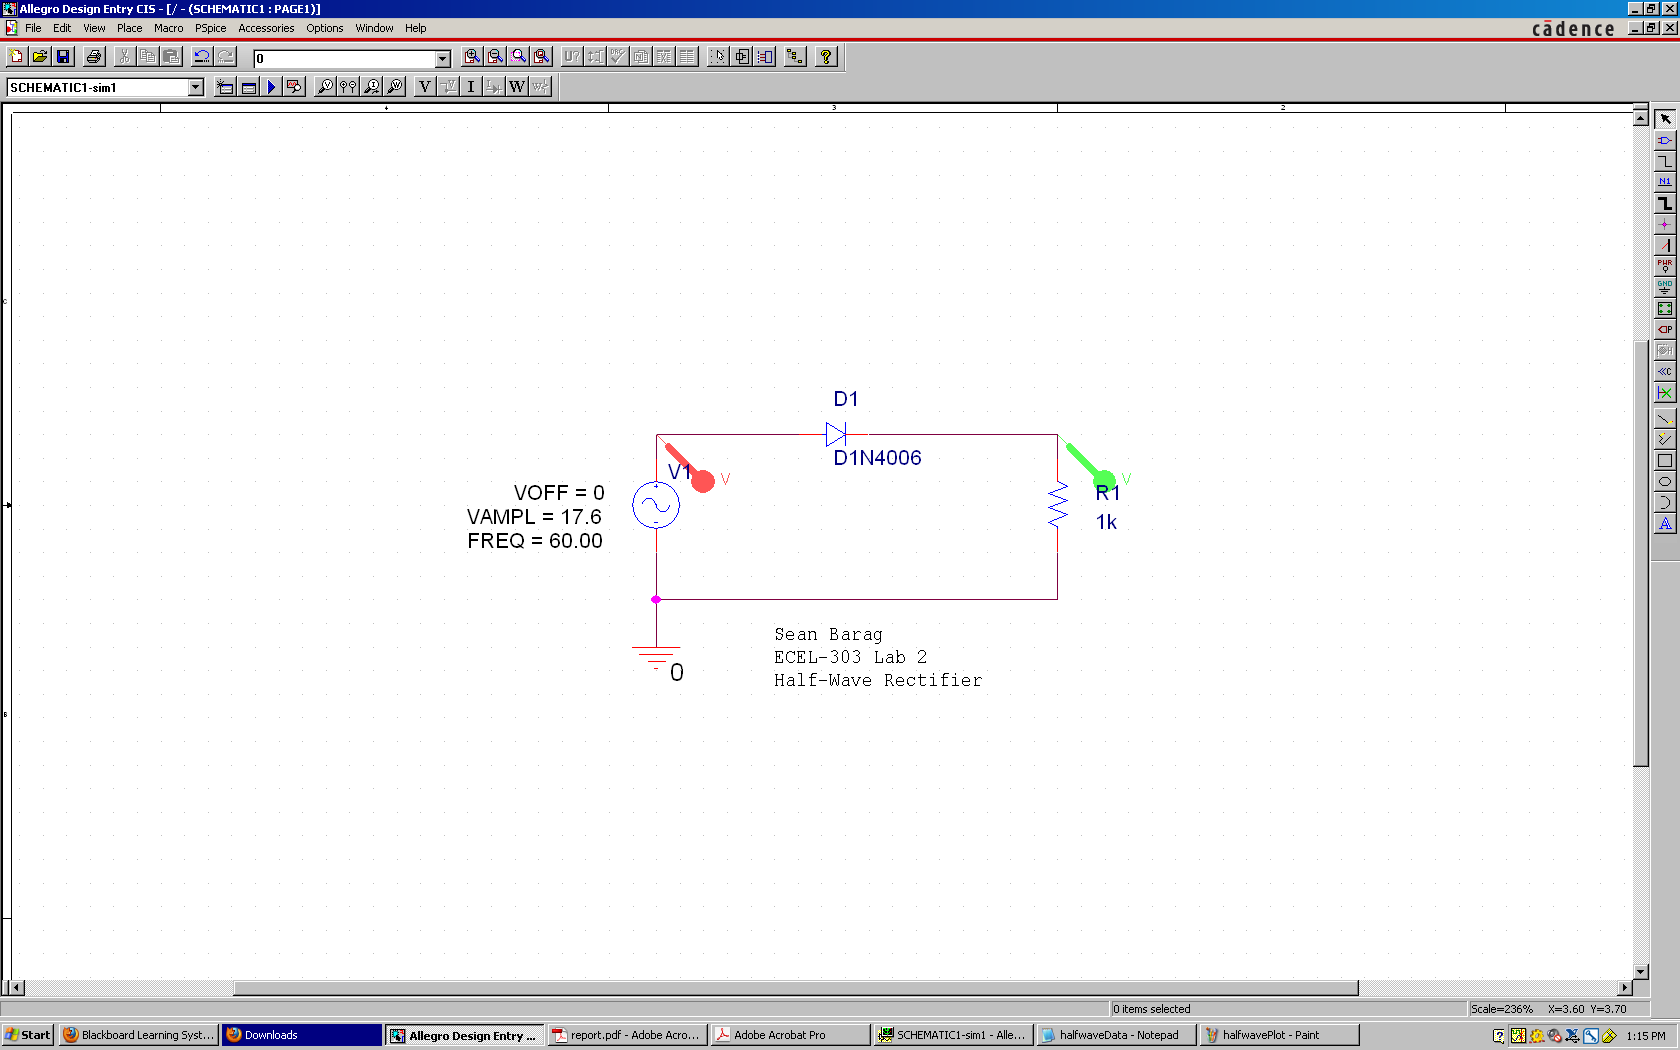
\includegraphics[width=.6\textwidth]{img/screen/halfwaveShot.PNG}
	\parbox{.6\textwidth}{
	\caption{Schematic capture of the half-wave rectifier shown initially in
		Figure~\ref{fig:schem1}.}
	\label{fig:pspice1}}
\end{figure}

\begin{figure}[H]
	\centering
	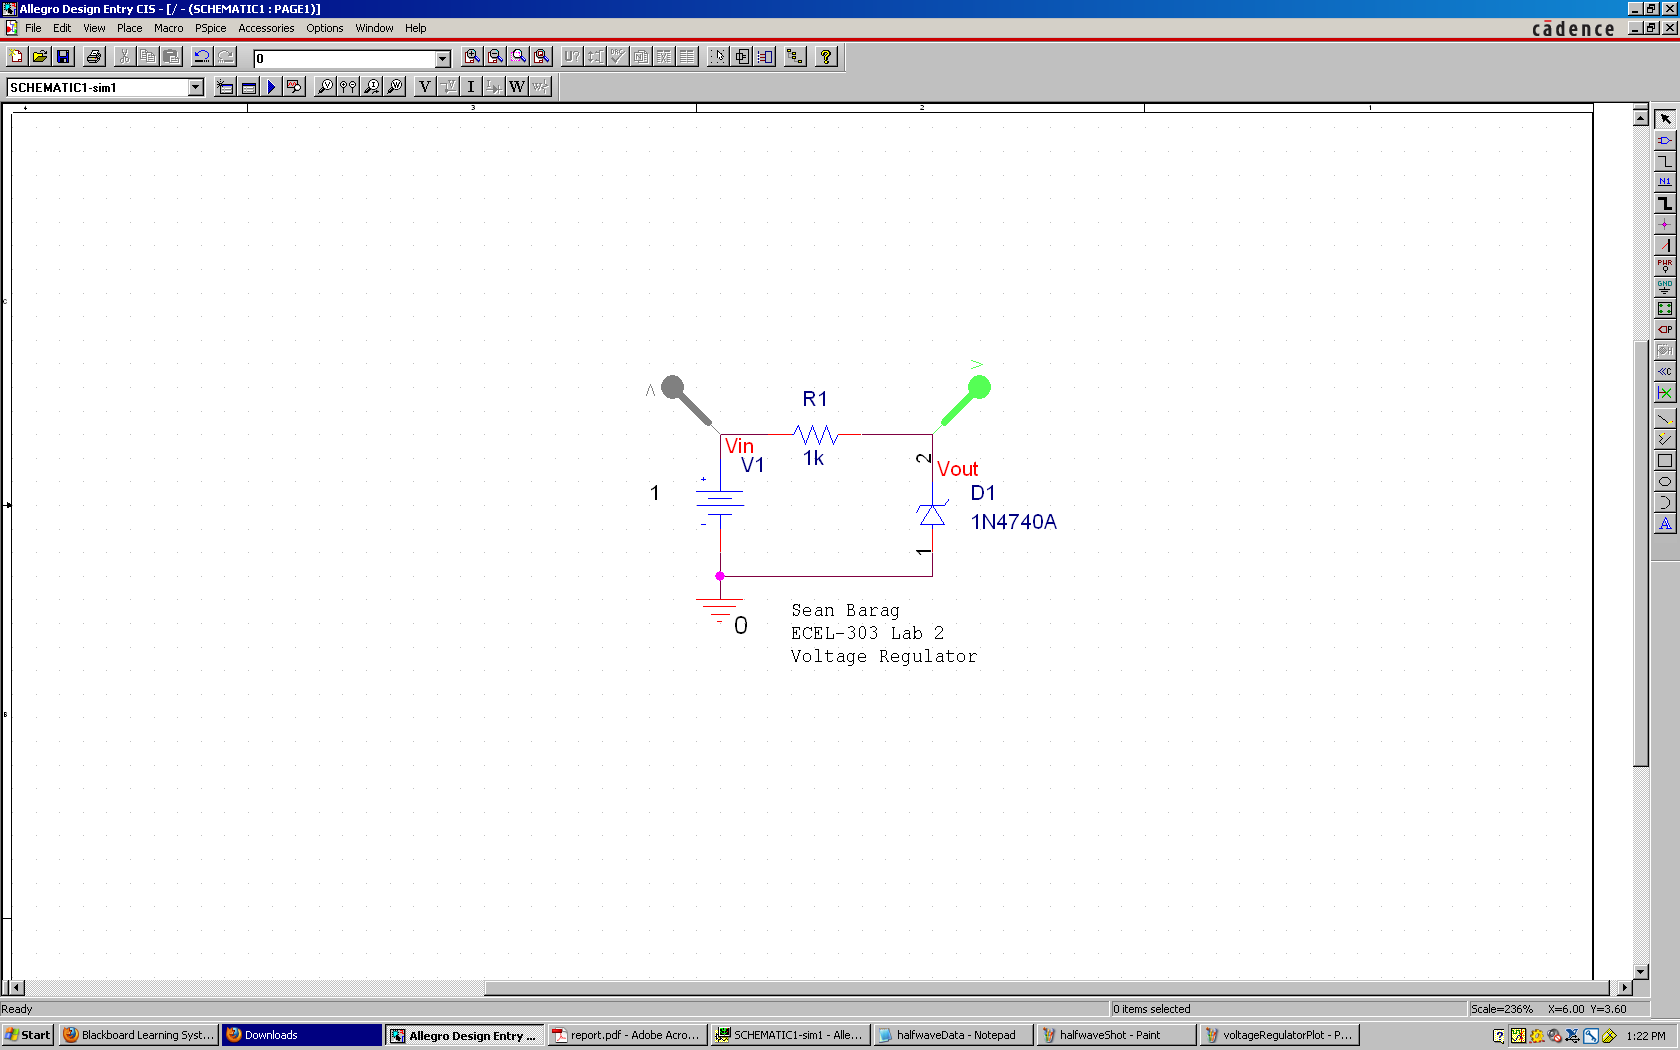
\includegraphics[width=.6\textwidth]{img/screen/voltageRegulatorShot.PNG}
	\parbox{.6\textwidth}{
	\caption{PSpice schematic for the DC voltage regulator originally drawn in
		Figure~\ref{fig:schem3}.}
	\label{fig:pspice3}}
\end{figure}

\begin{figure}[H]
	\centering
	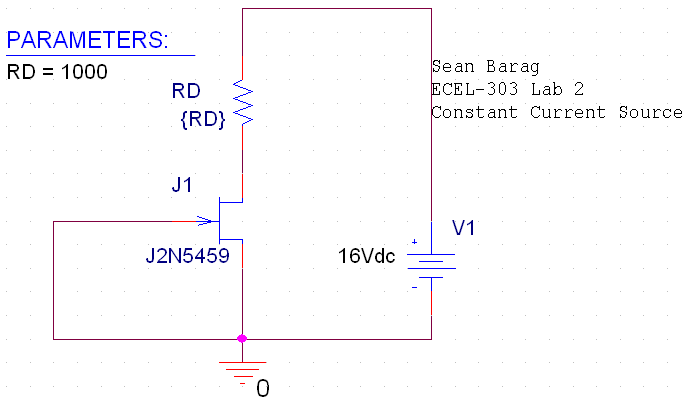
\includegraphics[width=.6\textwidth]{img/screen/constantCurrent16Shot.PNG}
	\parbox{.6\textwidth}{
	\caption{Simulated constant current source.  This circuit was originally
		presented in Figure~\ref{fig:schem4}, and has a counterpart circuit shown
		below in Figure~\ref{fig:pspice4b}.}
	\label{fig:pspice4a}}
\end{figure}

\begin{figure}[H]
	\centering
	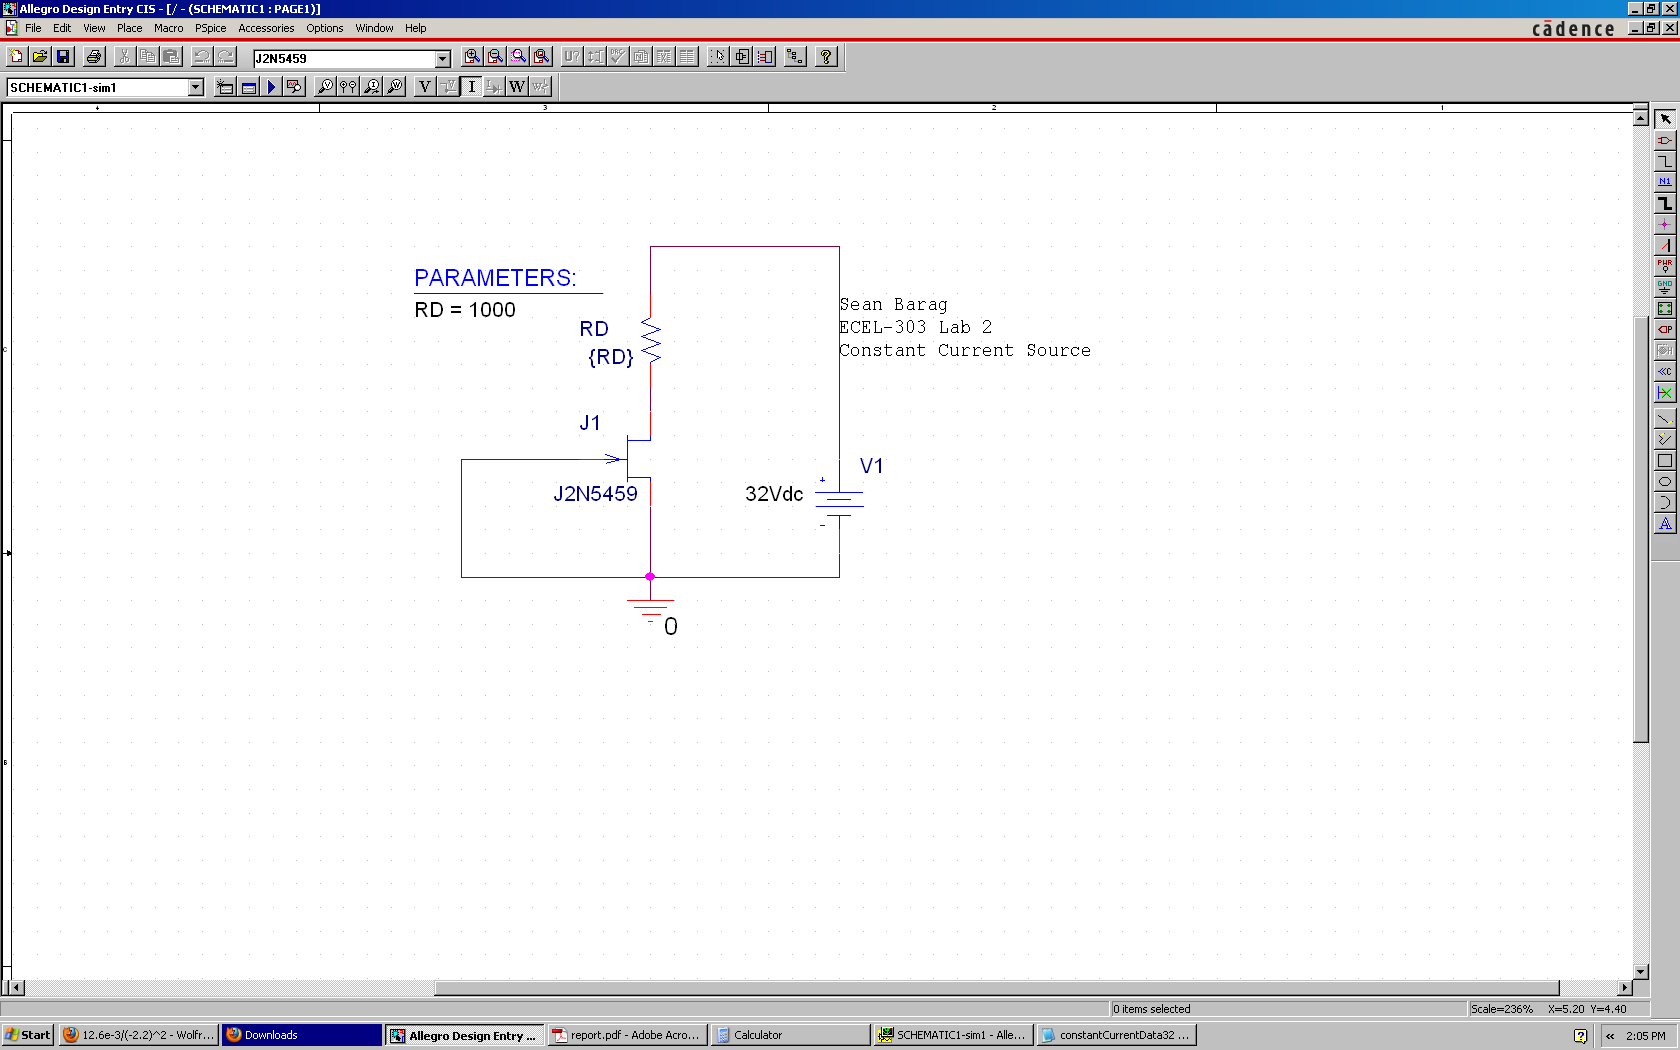
\includegraphics[width=.6\textwidth]{img/screen/constantCurrent32Shot.PNG}
	\parbox{.6\textwidth}{
	\caption{Companion circuit to the constant current source in
		Figure~\ref{fig:pspice4a}, originally drawn in Figure~\ref{fig:schem4}.
		Note the increased voltage from the DC source.}
	\label{fig:pspice4b}}
\end{figure}

\begin{figure}[H]
	\centering
	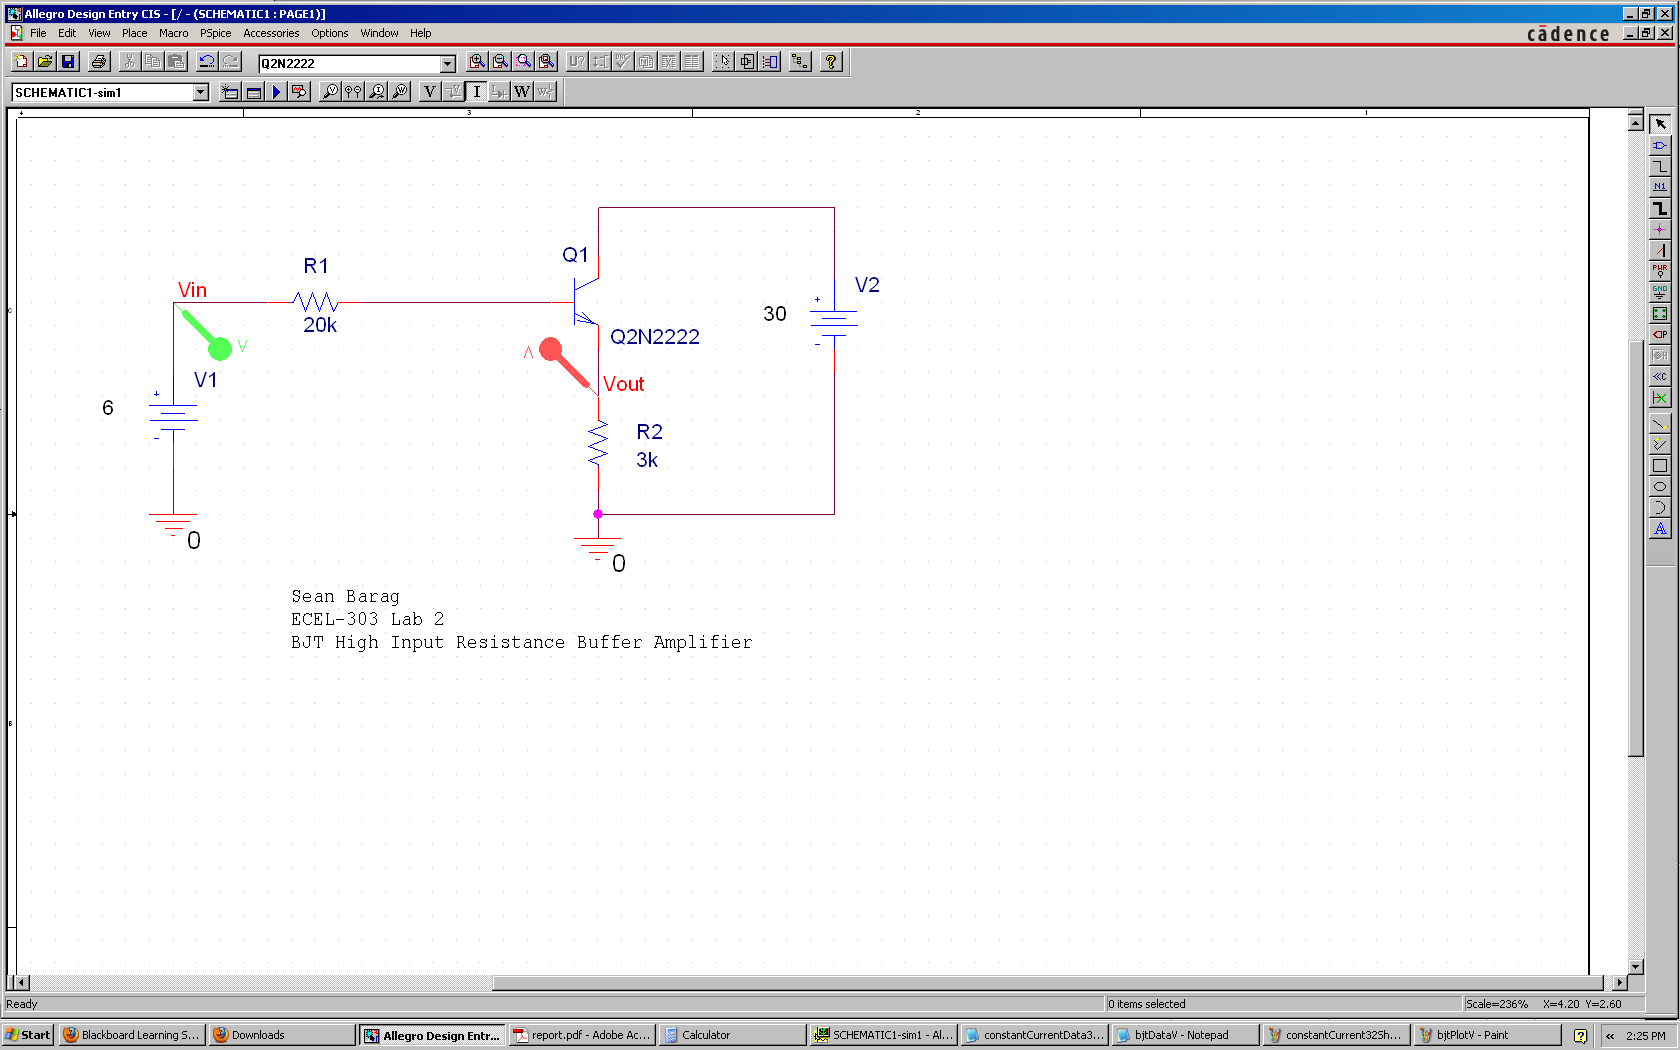
\includegraphics[width=.6\textwidth]{img/screen/bjtShot.PNG}
	\parbox{.6\textwidth}{
	\caption{Captured schematic of the BJT-based high input resistance buffer
		amplifier.  It was drawn initially in Figure~\ref{fig:schem5}.}
	\label{fig:pspice5}}
\end{figure}
